\chapter{Leveraging Bagging}
\label{ch:leveraging}


Bagging and Boosting are ensemble methods used to improve the accuracy of classifier methods. 
Non-streaming bagging~\cite{bagging} builds a set of  $M$ base models, training each model with a bootstrap sample of size $N$ created by drawing random samples with replacement from the original training set.  Each base model's training set contains each of the original training example $K$ times where $P(K=k)$ follows a binomial distribution. This binomial distribution  for large values of  $N$ tends to a Poisson(1) distribution, where  Poisson(1)$= \exp(-1)/k!$. Using this fact, Oza and Russell~\cite{ozabagboost,ozaexp} proposed {\em Online Bagging}, an online method that instead of sampling with replacement, gives each example a weight according to Poisson(1). 

Boosting algorithms combine multiple base models to obtain a small generalization error.
Non-streaming boosting builds a set of models sequentially, with the construction of each new model depending on the performance of the previously constructed models. The intuitive idea of boosting is to give more weight to misclassified examples, and reducing the weight of the correctly classified ones.

\BEGINOMIT
AdaBoost.M1~\cite{adaboost} generates a sequence of models using weighted training sets based on the performance of the previous model on the training set.  First, it creates a first model using the original training set, and it tests its accuracy on this training set. The weights of the correctly classified examples are scaled down, and the weights of the misclassified examples are scaled up.  The sum of the weight of the classified examples is the same as the misclassified examples. The next model is created using the learning algorithm with this new weight distribution on the training set. Doing that, some of the previously misclassified examples examples will be correctly classified by the new base model, because of their higher weights.
\ENDOMIT
%For online settings, Oza and Russell~\cite{ozabagboost,ozaexp} proposed {\em Online Boosting}, an online method that instead of building sequentially new models, each time a new instance arrive, it updates each model with a weight computed depending on the performance of the previous classifiers. 

From studies appearing in the literature~\cite{ozabagboost,ozaexp,ensemble},
Online Bagging seems to perform better than online boosting methods. Why bagging outperforms boosting in the data stream setting is still an open question. Adding more random weight to all instances seems to improve accuracy more than adding weight to misclassified instances. In this chapter %To improve the performance of bagging
 we focus on randomization as a powerful tool to increase accuracy and diversity when constructing an ensemble of classifiers.
There are three ways of using randomization:
\begin{itemize}
\item Manipulating the input data
\item Manipulating the classifier algorithms   
\item Manipulating the output targets
\end{itemize}
 
In this chapter we focus on randomizing the input data and the output prediction of online bagging.

\section{Bagging Literature}
\label{Rel}

Breiman~\cite{bagging} introduced bagging classification using the notion of an {\em order-correct} learner. An order-correct learner $\phi$ at the input $x$ is a predictor that if input $x$ results in a class more often than any other class, then $\phi$ will also predict this class at $x$ more often than any other class. An order-correct learner is not necessarily an accurate predictor but its aggregated predictor is optimal. If a predictor is good because it is order-correct for most inputs $x$ then aggregation can transform it into a nearly optimal predictor. The vital element to gain accuracy is the instability of the prediction method. A learner is unstable if a small change in the input data leads to large changes in the output.

Friedman~\cite{friedman} explained that bagging works by reducing variance without changing the bias. There are several definitions of bias and variance for classification, but the common idea is that bias measures average error over many different training sets, and variance measures the additional error due to the variation in the model produced by using different training sets.

Domingos~\cite{Domingos97} claimed that Breiman's line of reasoning is limited, since we may never know {\em a priori} whether a learner is order-correct for a given example or not, and what regions of the instance space will be order-correct or not. He explained bagging's success showing that bagging works by effectively changing a single-model learner to another single-model learner, with a different implicit prior distribution over models, one that is less biased in favor of simple models.

Some work in the literature shows that bagging asymptotically performs some smoothing on the estimate. Friedman and Hall~\cite{Friedman99onbagging} used an asymptotic truncated Taylor series of the estimate to show that in the limit of infinite samples, bagging reduces the variance of non-linear components.

B\"uhlmann and Yu~\cite{yu-bag}, analyzed bagging using also asymptotic limiting distributions, and they proposed {\em subagging} as a less expensive alternative to bagging. Subagging uses subsampling as an alternative aggregation scheme. They claimed that subagging is as accurate as bagging but uses less computation.


Grandvalet\cite{Grandvalet04} explained the performance of bagging by the goodness and badness of highly influential examples, in situations where the usual variance reduction argument is questionable. He presented an experiment showing that bagging increases the variance of decision trees, and claimed that bagging does not simply reduce variance in its averaging process.


In~Chapter~\ref{ch:ensemblemethods} two new state-of-the-art bagging methods were presented: ASHT Bagging using trees of different sizes, and \adwin Bagging using a change detector to decide when to discard underperforming 
ensemble members. 


\BEGINOMIT
\begin{algorithm}
\caption{Oza and Russell's {\em Online Bagging} for $M$ models} %in the ensemble }
\begin{algorithmic}[1]
\STATE Initialize base models $h_{m}$ for all $m \in \{1,2,...,M\}$
\FORALL{training examples}
\FOR{$m=1,2,...,M$}
\STATE Set $w = $ {\em Poisson}(1)
%\FOR{$n=1,2,...,k$}
\STATE Update $h_{m}$ with the current example with weight $w$
%\ENDFOR
\ENDFOR
\ENDFOR
\STATE {\bf anytime output:}
\RETURN hypothesis: $h_{fin}(x) = \arg \max_{y \in Y} \sum_{t=1}^{T} I(h_{t}(x) = y)$
\end{algorithmic}
\label{alg:ozabag}
\end{algorithm}
\ENDOMIT

%Boosting algorithms combine multiple base models to obtain a small generalization error.
%Non-streaming boosting builds a set of models sequentially, with the construction of each new model depending on the performance of the previous constructed models. The intuitive idea of boosting is to give more weight to the misclassified examples, and reduce the weight of the correctly classified ones.

%For online settings, Oza and Russell~\cite{ozabagboost,ozaexp} proposed {\em Online Boosting}, an online method that instead of building sequentially new models, each time a new instance arrive, it updates each model with a weight computed depending on the performance of the previous classifiers. %The pseudo-code is listed in Algorithm~\ref{alg:ozaboost}

Breiman~\cite{randomforests} proposed Random Forests as a method to use randomization on the input and on the internal construction of the decision trees. Random Forests are ensembles of trees with the following characteristics: the input training set is obtained by sampling with replacement, the nodes of the tree only may use a fixed number of random attributes to split, and the trees are grown without pruning. Abdulsalam et al.~\cite{Abdulsalam} presented a streaming version of random forests and Saffari et al.~\cite{SaffariORF2009} presented an online version.

\BEGINOMIT

\begin{algorithm}
\caption{Oza and Russell's {\em Online Boosting}.}
\begin{algorithmic}[1]
\STATE Initialize base models $h_{m}$ for all $m \in \{1,2,...,M\}, \lambda_{m}^{sc}=0, \lambda_{m}^{sw}=0$
\FORALL{training examples}
\STATE Set ``weight'' of example $\lambda_{d} = 1$
\FOR{$m=1,2,...,M$}
\STATE Set $w = $ {\em Poisson}($\lambda_{d}$)
%\FOR{$n=1,2,...,k$}
\STATE Update $h_{m}$ with the current example with weight $w$
%\ENDFOR
\IF{$h_{m}$ correctly classifies the example}
\STATE $\lambda_{m}^{sc} \gets \lambda_{m}^{sc} + \lambda_{d}$
\STATE  $\epsilon_{m} = \frac{\lambda_{m}^{sw}}{\lambda_{m}^{sc} + \lambda_{m}^{sw}}$
\STATE $\lambda_{d} \gets \lambda_{d} \left( \frac{1}{ 2( 1-\epsilon_m)} \right)$
\ELSE
\STATE $\lambda_{m}^{sw} \gets \lambda_{m}^{sw} + \lambda_{d}$
\STATE  $\epsilon_{m} = \frac{\lambda_{m}^{sw}}{\lambda_{m}^{sc} + \lambda_{m}^{sw}}$
\STATE $\lambda_{d} \gets \lambda_{d} \left( \frac{1}{2 \epsilon_m} \right)$
\ENDIF
\ENDFOR
\ENDFOR
\STATE {\bf anytime output:}
%\STATE Calculate  $\beta_{m} = \epsilon_{m} / (1 - \epsilon_{m})$ for all $m \in \{1,2,...,M\}$
\STATE Calculate  $\alpha_{m} = \log \frac{1 - \epsilon_{m}}{\epsilon_{m} } $ for all $m \in \{1,2,...,M\}$
\RETURN hypothesis: $h_{fin}(x) = \arg \max_{y \in Y} \sum_{m:h_{m}(x)=y} \alpha_{m} $
\end{algorithmic}
\label{alg:ozaboost}
\end{algorithm}

Breiman~\cite{arcing} 
proposed a simple boosting algorithm, {\em arc-x4}, to point out that the success of boosting may lay not in its specific form but in its adaptive resampling property: place increasing weight on those cases more frequently misclassified.  Arc-x4 uses an unweighted voting, and the weights used to train the models are based in the probabilities defined by

$$ p(n)= ( 1+ mc_{t}(n)^4)/ \sum(1+mc_{t}(n)^ 4)$$ 

where $mc_{t}(n)$ is the number of misclassifications of the models  $1$ to $t$ by example $n$.

The online version of {\em arc-x4} was proposed by Fern and Givan~\cite{onlinearcx4},. % and its pseudo-code is shown in Algorithm~\ref{alg:arcx4}. 
Note that they use a weighted voting strategy, but they claim that for ensemble sizes the two strategies give nearly identical results. Online arcx-4 has three steps: first it updates the vote of the model, second it computes the weight using the number of misclassification of the previous models, and finally, it trains the model with the weight calculated in the second step.



Breiman~\cite{ivotes} proposed an arcing on-line method {\em Ivotes} using the idea of importance voting. As a new example arrive, it is checked to see how it is classified by the current classifier. If misclassified it is accepted with a weight of one. If not, it is accepted with probability $e_T/(1-e_T)$, where the error estimate $e_T$ is computed as a smoothed version of the proportion of misclassified examples.
\ENDOMIT
\BEGINOMIT
\begin{algorithm}
\caption{Fern and Givan's {\em Online Arc-x4} for $M$ models} %in the ensemble }
\begin{algorithmic}[1]
\STATE Initialize base models $h_{m}$ for all $m \in \{1,2,...,M\}, v_{m} = 0$
\FORALL{training examples}

\FOR{$m=1,2,...,M$}
\IF{$h_{m}$ correctly classifies the example}
\STATE $v_{m} \gets v_{m}+1$
\ENDIF
\STATE $mc_t = 0$
\FOR{$t=1,2,...,m-1$}
\IF{$h_{t}$ correctly classifies the example}
\STATE $mc_t \gets mc_t +1$
\ENDIF
\ENDFOR
\STATE Set $w =  1 + mc_{t}^{4}$ %{\em Poisson}(1)
%\FOR{$n=1,2,...,k$}
\STATE Update $h_{m}$ with the current example with weight $w$
%\ENDFOR
\ENDFOR
\ENDFOR
\STATE {\bf anytime output:}
\RETURN hypothesis: $h_{fin}(x) = \arg \max_{y \in Y} \sum_{m:h_{m}(x)=y} v_{m}$
\end{algorithmic}
\label{alg:arcx4}
\end{algorithm}


Zhu et al.~\cite{multiclassadaboost} presented SAMME as a multi-class version of AdaBoost.M1, as AdaBoost.M1 has a strong restriction for multi-class problems: the error of each classifier has to be less than $1/2$. They presented SAMME as a method with the same simple modular structure of AdaBoost.M1, but with an important difference: the addition of the term $\log (K-1)$ to the weight $\alpha_m$ of the $m$ classifier, where $K$ is the number of classes:

$$\alpha_{m} = \log \frac{1 - \epsilon_{m}}{\epsilon_{m} } + \log (K-1)$$
 
 For two classes, the term  $\log (K-1)$ t is zero, and SAMME reduces to AdaBoost.M1. 

\ENDOMIT
\section{Leveraging Bagging}
\label{Per}

In this section, we present a new online leveraging bagging algorithm, improving Online Bagging of  Oza and Russell.
The pseudo-code of Online Bagging of Oza and Russell 
is listed in Algorithm~\ref{alg:ozabag}.

We leverage the performance of bagging, with two randomization improvements: increasing resampling and using output detection codes.


\begin{algorithm}
\caption{{\em Leveraging  Bagging} for $M$ models} %in the ensemble }
\begin{algorithmic}[1]
\STATE Initialize base models $h_{m}$ for all $m \in \{1,2,...,M\}$
\STATE Compute coloring $\mu_m(y)$
\FORALL{training examples $(x,y)$}
%\STATE $mc = 0$
%\FOR{$m=1,2,...,M$}
%\IF{$h_{m}$ correctly classifies the example}
%\STATE $mc \gets mc +1$
%\ENDIF
%\ENDFOR
\FOR{$m=1,2,...,M$}
\STATE Set $w = $ {\em Poisson}($\lambda$)
%\FOR{$n=1,2,...,k$}
\STATE Update $h_{m}$ with the current example with weight $w$ and class $\mu_m(y)$
%\ENDFOR
\ENDFOR
\ENDFOR
\IF{\adwin  detects change in error of one of the classifiers}
\STATE Replace classifier with higher error with a new one 
\ENDIF
\STATE {\bf anytime output:}
\RETURN hypothesis: $h_{fin}(x) = \arg \max_{y \in Y} \sum_{t=1}^{T} I(h_{t}(x) =\mu_t( y))$
\end{algorithmic}
\label{alg:levbag}
\end{algorithm}
 

 Resampling with replacement is done in Online Bagging using Poisson(1). 
 There are other sampling mechanisms:
 \begin{itemize}
\item    Lee and Clyde~\cite{bayesian} uses the Gamma distribution (Gamma(1,1)) to obtain a Bayesian version of Bagging. Note that Gamma(1,1) is equal to Exp(1). 
\item Bulhman and Yu~\cite{yu-bag} proposes subagging, using resampling without replacement. 
\end{itemize}

  
  \begin{figure}[h]
\begin{center} 
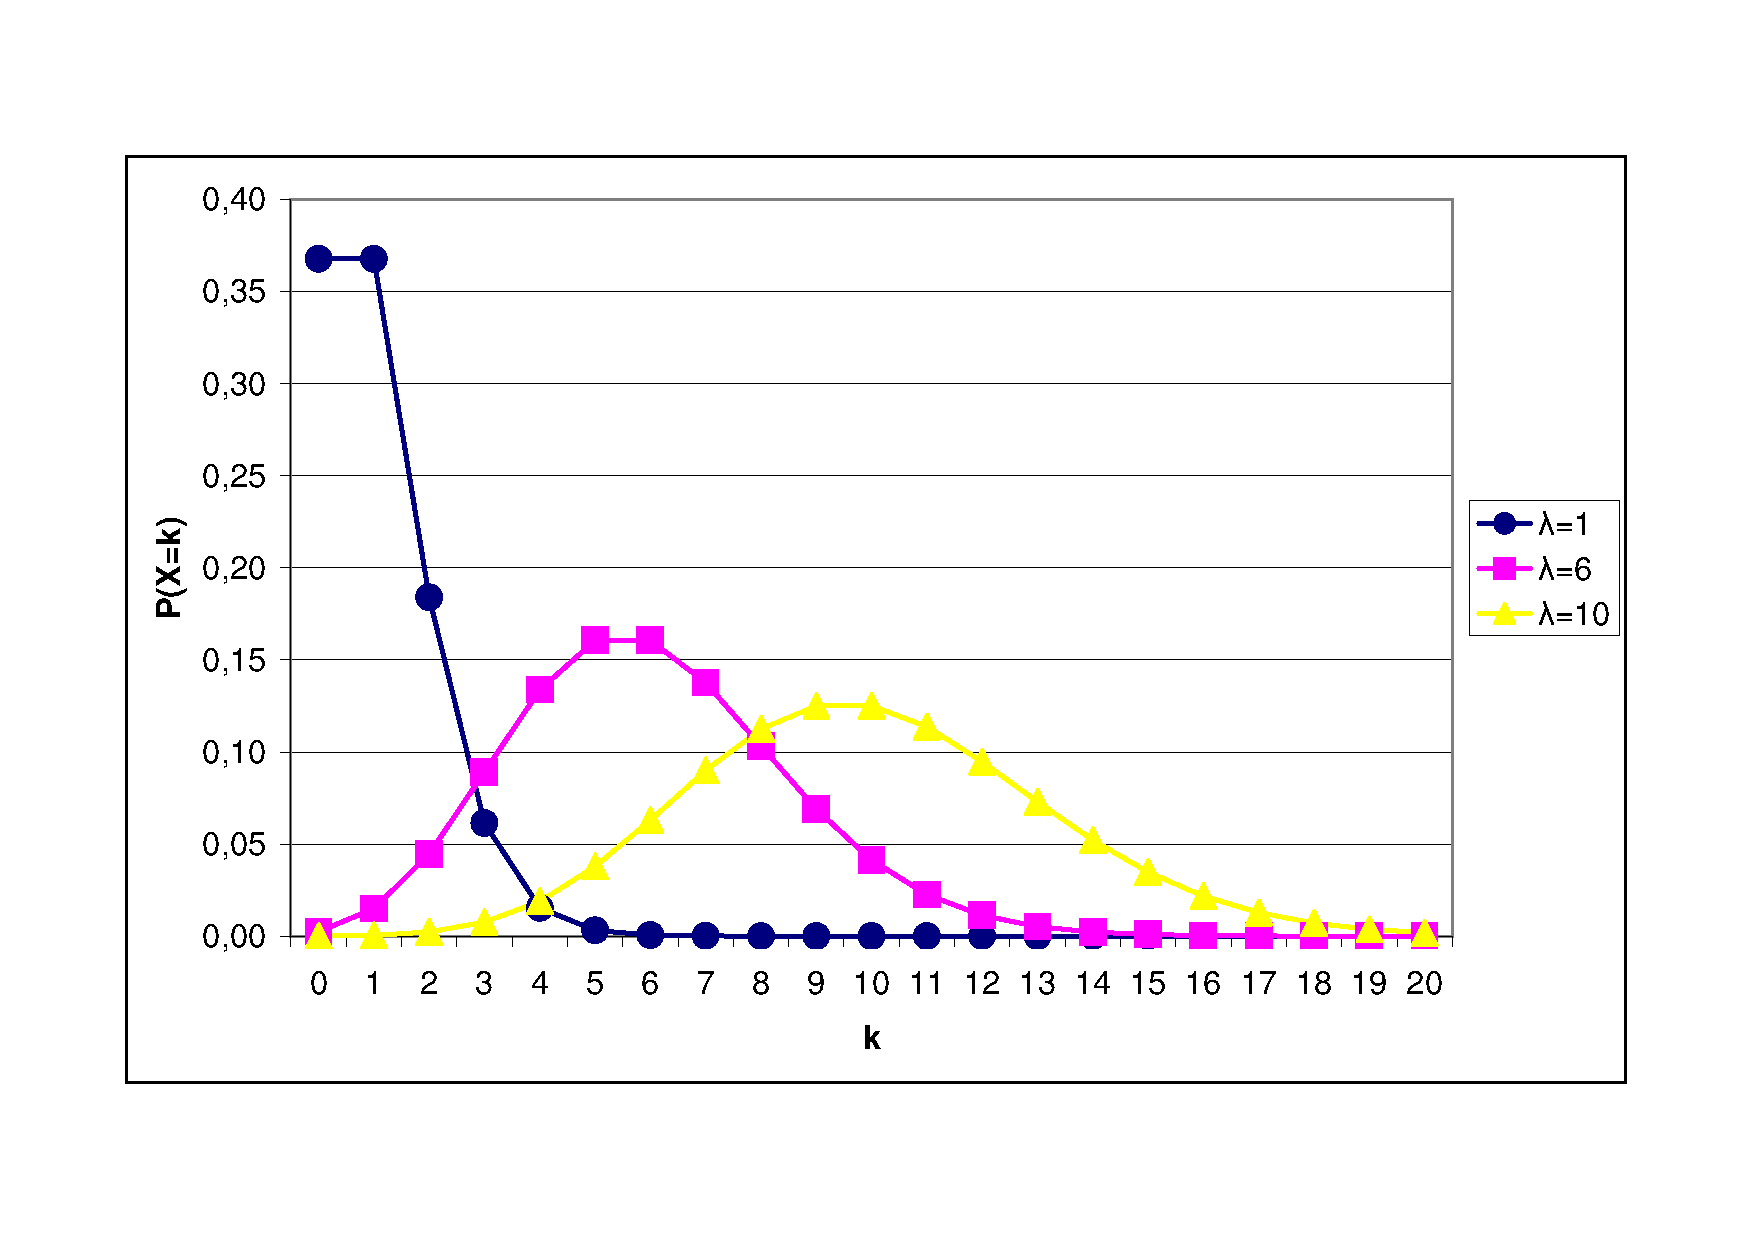
\epsfig{file=figures/Poisson.pdf, scale=.4}%9} 

\end{center}
\caption{Poisson Distribution.}

\label{fig:poisson}
\end{figure}
 Our proposal is to increase the weights of this resampling using a larger value $\lambda$ to compute the value of the Poisson distribution.  
The Poisson distribution is used to model the number of events occurring within a given time interval. 

Figure~\ref{fig:poisson} shows the probability function mass of the distribution of Poisson for several values of $\lambda$. The mean and variance of a Poisson distribution is $\lambda$.  
For $\lambda=1$ we see that $37\%$ of the values are zero, $37\%$ are one, and $26\%$ are values greater than one. Using a weight of Poisson(1) we are taking out   $37\%$ of the examples, and repeating $26\%$ of the examples, in a similar way to non streaming bagging.
For $\lambda=6$ we see that $0.25\%$ of the values are zero, $45\%$ are lower than six, $16\%$ are six, and $39\%$ are values greater than six.  Using a  value of $\lambda > 1$ for Poisson($\lambda$) we are increasing the diversity of the weights and modifying the input space of the classifiers inside the ensemble. However, the optimal value of $\lambda$ may be different for each dataset. 
  
 Our second improvement is to add randomization at the output of the ensemble using output codes. Dietterich and Bakiri~\cite{ecoc} introduced a method based on error-correcting output codes, which handles multiclass problems using only a binary classifier. The classes assigned to each example are modified to create a new binary classification of the data induced by a mapping from the set of classes to \{0,1\}. A variation of this method by Schapire~\cite{BoostOC} presented a form of boosting using output codes.
 
 We assign to each class a binary string of length $n$ and then build an ensemble of $n$ binary classifiers. Each of the classifiers learns one bit for each position in this binary string. When a new instance arrives, we assign $x$ to the class whose binary code is closest. We can view an error-correcting code as a form of voting in which a number of incorrect votes can be corrected.
 
We use random output codes instead of deterministic codes. In standard ensemble methods, all classifiers try to predict the same function. However, using output codes each classifier will predict a different function. This may reduce the effects of correlations between the classifiers, and increase diversity of the ensemble.

We implement random output codes in the following way: we choose for each classifier $m$ and class $c$ a binary value $\mu_m(c)$ in a uniform, independent, and random way. We ensure that exactly half of the classes are mapped to $0$. The output of the classifier for an example is the class which has more votes of its binary mapping classes. Table~\ref{tab:codes} shows an example for an ensemble of 6 classifiers in a classification task of 3 classes. 
 
 \begin{table}[h]
\caption{Example matrix of random output codes for 3 classes and 6 classifiers}
 \begin{center}
  \begin{tabular}{| l | c | c | c | }
    \hline
     &  Class 1 & Class 2 & Class 3  \\ \hline
   Classifier 1 & 0 & 0 & 1  \\ 
   Classifier 2 & 0 & 1 & 1  \\ 
   Classifier 3 & 1 & 0 & 0  \\
   Classifier 4 & 1 & 1 & 0  \\
   Classifier 5 & 1 & 0 & 1  \\
   Classifier 6 & 0 & 1 & 0  \\
    \hline
  \end{tabular}
\end{center}
\label{tab:codes}
\end{table}%

 
We use the same strategy as in Chapter~\ref{ch:ensemblemethods}.
\adwinb~\cite{bif-gav} is a change detector and estimator that solves in a 
well-specified way the problem of tracking the average of a stream of bits or 
real-valued numbers. \adwin keeps a variable-length window of recently seen 
items, with the property that the window has the maximal length statistically 
consistent with the hypothesis ``there has been no change in the average value
inside the window". 

\BEGINOMIT
More precisely, an older fragment of the window is dropped if and only if 
there is enough evidence that its average value differs from that of 
the rest of the window. 
This has two consequences: one, that change reliably declared whenever
the window shrinks; and two, that at any time the average over the existing
window can be reliably taken as an estimation of the current average in the stream
(barring a very small or very recent change that is still not statistically 
visible). A formal and quantitative statement of these two points (a theorem)
appears in \cite{bif-gav}. 
\ENDOMIT

\adwin is parameter- and assumption-free in the sense that 
it automatically detects and adapts to the current rate of change. 
Its only parameter is a confidence bound $\delta$,
indicating how confident we want to be in the algorithm's output, 
inherent to all algorithms dealing with random processes. 

Also important for our purposes, \adwin does not maintain the window
explicitly, but compresses it using a variant of the exponential histogram
technique. % in \cite{babcock-sampling}. 
This means that it keeps a window of length $W$
using only $O(\log W)$ memory and $O(\log W)$ processing time per item. %, 


Algorithm~\ref{alg:levbag} shows the pseudo-code of our Leveraging Bagging.
First we build a matrix with the values of $\mu$ for each classifier and class. 
For each new instance that arrives,  we give it a random weight of $Poisson(k)$.
We train the classifier with this weight,
and when a change is detected, the worst classifier of the ensemble of classifiers 
is removed and a new classifier is added to the ensemble.
To predict the class of an example, we compute for each class $c$ the sum of the votes for $\mu(c)$ of all the ensemble classifiers, and we output as a prediction the class with the most votes.


